\documentclass[12pt,a4paper,titlepage]{article}
\title{Simulations of Monolayer and Multilayer MoS$_2$ FET} 
\author{Matteo Orlandini \& Jacopo Pagliuca}
\date{}

\usepackage[italian, english]{babel} %the last declared language is the one used in the document
\usepackage[utf8]{inputenc}
\usepackage[T1]{fontenc}
\usepackage{amsmath}
\usepackage{amssymb}
\usepackage{subfig}
\usepackage{graphicx}
\usepackage{listings}
\usepackage{booktabs}
%inizio impostazioni bibliografia
\usepackage[autostyle,italian=guillemets]{csquotes} 
%autostyle adatta lo stile delle citazioni alla lingua corrente del documento;
%italian=guillemets racchiude automaticamente tra virgolette caporali
%i campi che prevedono le virgolette;
\usepackage[backend=biber, style=numeric, citestyle=numeric,maxcitenames=99,maxbibnames = 99]{biblatex}
%backend=biber dice a biblatex che s’intende usare Biber come motore bibliografico
%style:numeric Anno di pubblicazione: in fondo al riferimento.
%citestyle=numeric Riferimento: numerico ([1], [2], eccetera).
%fine impostazioni bibliografia

\usepackage{float}
\usepackage{hyperref}
\hypersetup{
	bookmarks=true,         % show bookmarks bar?
	unicode=false,          % non-Latin characters in Acrobat’s bookmarks
	pdftoolbar=true,        % show Acrobat’s toolbar?
	pdfmenubar=true,        % show Acrobat’s menu?
	pdffitwindow=false,     % window fit to page when opened
	pdfstartview={FitH},    % fits the width of the page to the window
	%pdftitle={Relazione di Reti di Sensori Wireless per IOT},    % title
	pdfauthor={Matteo Orlandini},     % author
	pdfsubject={Simulations of Monolayer and Multilayer MoS$_2$ FET}  % subject of the document
	pdfcreator={Matteo Orlandini},   % creator of the document
	%pdfproducer={Producer}, % producer of the document
	pdfpagemode={UseOutlines},
	%bookmarksopen,
	pdfpagelabels=true
	pdfstartview={FitH},
	colorlinks=false,       % false: boxed links; true: colored links
	linkcolor={red},
	citecolor={green},
	urlcolor={cyan},
} 


\addbibresource{Bibliography.bib}

\newcommand{\CoverName}{Cover}

\begin{document}
\renewcommand{\thepage}{\CoverName}
\begin{titlepage}
	
	\centering
	\includegraphics[width=.2\textwidth]{Immagini/univpmlogo}\par\vspace{1cm}
	{\scshape\LARGE Università Politecnica delle Marche\par}
	\vspace{1cm}
	{\scshape\Large Multiphysics Systems for Radio Frequency Electronics\par}
	\vspace{1.5cm}
	{\huge\bfseries  Simulations of Monolayer and Multilayer MoS$_2$ FET \par}
	\vspace{2cm}
	{\Large\itshape Matteo Orlandini \par}
	{\Large\itshape Jacopo Pagliuca\par}
	\vfill
	supervised by\par
	Prof. Davide \textsc{Mencarelli}, Prof. Luca \textsc{Pierantoni}\\ and Nicola \textsc{Pelagalli}
	
	\vfill
	
	% Bottom of the page
	{\large \today\par}
\end{titlepage}

\thispagestyle{empty}
\pagenumbering{roman}
\tableofcontents

\newpage
\pagenumbering{arabic}
\setcounter{page}{1}
\section{Introduction}
Two dimensional materials are object of researches due to their ease to fabricate complex structures with them and the high performance that they show.
We use MoS$_2$ 2-D layers over graphene because of the intrinsic bandgap of 1.8 eV. In the graphene this bandgap is absent and it can be engineered with complex methods.
A single layer of MoS$_2$ can be substituted to a transistor channel.
In the following report different kinds of models of transistors based on the monolayer material have been studied.
They are based on a silicon substrate under a SiO$_2$ layer that isolate the bottom gate from the 2-D material that acts like a channel. The latter is connected to two metal contacts that have the roles of source and gate.
The first model is a simple transistor with a single silicon bottom gate based on the one in~\cite{Howell:MonolayerMultiLayer_MoS2}, studied with one and four monolayers.
Another one has also a top gate made of Cr/Au isolated by a layer of hafnium dioxide like in~\cite{Radisavljevic:Si_MoS2}.
We use a hafnium dioxide gate dielectric to demonstrate a room-temperature single-layer MoS$_2$ mobility of at least $200~cm^2 V^{-1} s^{-1}$, similar to that of graphene nanoribbons.
The last model contains a ferroelectric material under the MoS$_2$ with a permittivity that changes with the voltage as an addition variable.
We have implemented all the models in COMSOL Multiphysics using the parameters shown in the table~\ref{table:MoS2} and~\ref{table:HfO2}. The results obtained are then compared with the experimental ones found in~\cite{Howell:MonolayerMultiLayer_MoS2} and~\cite{Radisavljevic:Si_MoS2}. The physics used is the semiconductor one given by COMSOL Multiphysics.
Our models seems to simulate quite correctly the technology, in facts the plots obtained are very similar with the ones found in literature.
We can therefore say that they can be used for further experiments and expect that the results will be similar to the real ones.

\newpage
\section{MoS$_2$ transistor}

In~\cite{Howell:MonolayerMultiLayer_MoS2} is investigated the band-offsets at monolayer-multilayer MoS$_2$ junctions by scanning photocurrent microscopy. The thickness-dependent band structure of MoS$_2$ implies that discontinuities in energy bands exist at the interface of monolayer (1L) and multilayer (ML) thin films. The characteristics of such heterojunctions are analyzed using finite element simulations of charge carrier transport. We used that simulations to compare their results to our COMSOL model.

Transition metal dichalcogenides (TMDCs) such as MoS$_2$ consist of discrete two-dimensional (2D) layers bound together by van der Waals forces, with important consequences for both physical and electronic structure of these ultrathin semiconducting crystals. MoS$_2$ flakes exhibit distinctive thickness-dependent variations in physical properties and the band structure varies with multilayer thickness.

MoS$_2$ flakes were exfoliated from commercially available crystals of molybdenite onto n$^+$ Si substrates coated with 300 nm of SiO$_2$. The devices were formed by electron beam lithography and lift-off of Au ohmic contacts with 75 nm thickness. Fig.~\ref{fig:monolayer_model} shows the device geometry.
%\begin{figure}[H]
%	\centering
%	\subfloat[][Monolayer model~\cite{Wu:Ultrathin_MoS2}]
%	{\includegraphics[width=.45\textwidth]{Immagini/monolayer_model.png} \label{fig:monolayer_model}}
%	\subfloat[][COMSOL monolayer model]
%	{\includegraphics[width=.5\textwidth]{Immagini/monolayer_model_comsol.png} \label{fig:monolayer_model_comsol}} 
%\end{figure} 

\begin{figure}[H]
	\centering
	\includegraphics[width=.5\textwidth]{Immagini/monolayer_model.png} 
	\caption{Monolayer model~\cite{Wu:Ultrathin_MoS2}}
	\label{fig:monolayer_model}
\end{figure} 

The first step through implementing the model in COMSOL Multiphysics was defining the geometry: setting all the sizes and the distances between the materials. Later we specified which materials to associate with the different spatial regions and, for each one of them, we assigned all the physical variables necessary for the equations. We used a table of parameters for the materials defined in~\cite{Howell:MonolayerMultiLayer_MoS2}.

The next step was defining the physics. We used the semiconductor physic that implement the Poisson equation $\nabla \cdot (-\varepsilon_0 \varepsilon_r \nabla V) = \rho$. This physic allows us to specify the MoS$_2$ characteristics and to define the contacts of source, drain and gates. We defined the charge conservation and its equation $\vec{D} = \varepsilon_0 \varepsilon_r \vec{E}$ in the whole model except for the 2D material. The MoS$_2$ is treated like a semiconductor material model so we needed to specify the relative permittivity, the band gand, the electron affinity, the effective density of states in valence and conduction band and the electron and hole mobility in the material properties. Using analytic doping model we could set the donor concentration in the MoS$_2$ layer. The donor concentration is a parameter and it's varied in our studies according to the plot shown in~\cite{Howell:MonolayerMultiLayer_MoS2}. We used a trap assisted recombination to set the electron and hole lifetime according to Tab.~\ref{table:MoS2}. 

The mesh generated automatically was acceptable and precise enough. At last we created the studies that generated the plots in this report, trying to imitate the simulated ones found in~\cite{Howell:MonolayerMultiLayer_MoS2}.

\begin{figure}[H]
	\centering
	\includegraphics[width=.7\textwidth]{Immagini/monolayer_model_comsol.png}
	\caption{COMSOL monolayer model}
	\label{fig:monolayer_model_comsol}
\end{figure} 

The parameters used in COMSOL are shown in Tab.~\ref{table:MoS2}.

\begin{table}[H]
	\centering
	\begin{tabular}{l l}
		\toprule
		\textbf{Parameter}	       & \textbf{Value}			 \\
		\midrule
		Thickness of MoS$_2$       & 0.7nm/layer              \\
		Band gap 1L MoS$_2$        & 2.76 eV                  \\
		Band gap 4L MoS$_2$        & 1.6 eV                   \\
		Electron affinity 1L Mo$_2$& 4.7                      \\
		Electron affinity 4L MoS$_2$& 4                       \\
		Relative permittivity 1L   & 4.2                      \\
		Relative permittivity 4L   & 11                       \\
		Mobility 1L                & 6 $cm^2 V^{-1} s^{-1}$	  \\
		Mobility 4L                & 25 $cm^2 V^{-1} s^{-1}$  \\
		Drain contact type         & Ideal ohmic              \\
		Source contact type        & Ideal ohmic              \\
		SRH lifetimes 1L           & 1.5 ns                   \\
		SRH lifetimes 4L           & 0.3 ns                   \\
		Workfunction of gate       & 4.05 V                   \\
		SiO$_2$ Relative Permittivity & 3.9                   \\
		Electron effective mass    & $0.5 m_0$            	  \\
		Hole effective mass        & $0.5 m_0$           	  \\
		Thickness gold contact     & 75 nm                    \\
		Length MoS$_2$             & 3.5 $\mu m$              \\
		Silicon thickness          & 2 $\mu m$                \\
		SiO$_2$ thickness          & 300 nm	                  \\
		Width                      & 6.8 $\mu m$              \\
		\bottomrule
	\end{tabular}
	\caption{Parameters}
	\label{table:MoS2}
\end{table}

The figures shown below are the simulated and experimental (see legend) output characteristics when $V_G = 0.1 V$ (\ref{fig:4layer_Id(Vd)}) and transfer characteristics when $V_D = 0.01 V$ (\ref{fig:4layer_Id(Vg)})for a 4L thick FET. Simulated and experimental output characteristics when $V_G = 10 V$ (\ref{fig:monolayer_Id(Vd)}) and transfer characteristics when $V_D = 0.05$ (\ref{fig:monolayer_Id(Vg)}) for a 1L thick FET. Experimental data in are reproduced from~\cite{Wu:Ultrathin_MoS2}. Ideal transistor transfer curves show zero current below the threshold voltage and a linear gate bias dependence above the threshold voltage. Deviations of experimental transfer curves from ideal simulations have been attributed to scattering from unscreened charged impurities and a carrier density-dependent mobility. Mobility limited by Coulomb scattering leads to approximately parabolic instead of linear experimental transfer curves above the threshold voltage and reduces current magnitudes. An additional series contact resistance may further limit the current magnitudes in the experimental devices.

\begin{figure}[H]
	\centering
	\includegraphics[width=.8\textwidth]{Grafici/monolayer_Id(Vd).eps} 
	\caption{Monolayer $I_d(V_d)$}
	\label{fig:monolayer_Id(Vd)}
\end{figure}

\begin{figure}[H]
	\centering
	\includegraphics[width=.8\textwidth]{Grafici/monolayer_Id(Vg).eps} 
	\caption{Monolayer $I_d(V_g)$}
	\label{fig:monolayer_Id(Vg)}
\end{figure}

\begin{figure}[H]
	\centering
	\includegraphics[width=1\textwidth]{Grafici/4layer_Id(Vd).eps} 
	\caption{4 layer $I_d(V_d)$}
	\label{fig:4layer_Id(Vd)}
\end{figure}

\begin{figure}[H]
	\centering
	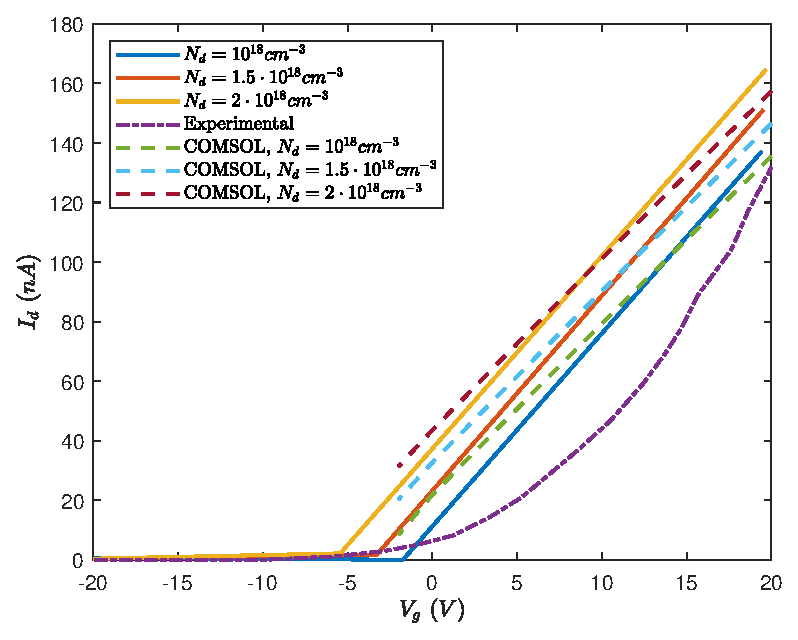
\includegraphics[width=.8\textwidth]{Grafici/4layer_Id(Vg).eps} 
	\caption{4 layer $I_d(V_g)$}
	\label{fig:4layer_Id(Vg)}
\end{figure}

\newpage
\section{MoS$_2$ transistor with HfO$_2$}
%\begin{figure}[H]
%	\centering
%	\subfloat[][HfO$_2$ model~\cite{Radisavljevic:Si_MoS2}]
%	{\includegraphics[width=.55\textwidth]{Immagini/HfO2_model.png} \label{fig:HfO2_model}}
%	\subfloat[][COMSOL HfO$_2$ model]
%	{\includegraphics[width=.45\textwidth]{Immagini/HfO2_model_comsol.png} \label{fig:HfO2_model_comsol}} 
%\end{figure} 
In~\cite{Radisavljevic:Si_MoS2} is studied a FET with a 30 nm HfO$_2$ top gate insulator. Using recent theoretical studies of mobility improvement by dielectric screening and its successful application to graphene, is used an atomic layer deposition (ALD) of 30 nm HfO$_2$ as a high-k gate dielectric for the
local top gate and mobility booster to realize the full potential of the single-layer MoS$_2$. HfO$_2$ is used because of its high dielectric constant of 25, bandgap of 5.7 eV and the fact that it is commonly used as a gate dielectric both by the research community and major microprocessor manufacturers. A schematic depiction of the device is shown in Fig.~\ref{fig:HfO2_fabrication}. The width of the top gate of this device is 4 $\mu m$ and the top gate length, source–gate and gate–drain spacing were 500 nm.

\begin{figure}[H]
	\centering
	\includegraphics[width=1\textwidth]{Immagini/HfO2_fabrication.png} 
	\caption{Three-dimensional schematic view of the transistor.~\cite{Radisavljevic:Si_MoS2}}
	\label{fig:HfO2_fabrication}
\end{figure} 

\begin{figure}[H]
	\centering
	\includegraphics[width=1\textwidth]{Immagini/HfO2_model.png} 
	\caption{Cross sectional view of the structure of a monolayer MoS$_2$ FET together with electrical connections used to characterize the device. A single layer of MoS$_2$ (thickness, 6.5 \AA) is deposited on a degenerately doped silicon substrate with 270-nm-thick SiO$_2$. The substrate acts a back gate. One of the gold electrodes acts as drain and the other source electrode is grounded. The monolayer is separated from the top gate by 30 nm of ALD-grown HfO$_2$. The top gate width for the device is 4 $\mu m$ and the top gate length, source–gate and gate–drain spacing are each 500 nm.~\cite{Radisavljevic:Si_MoS2}}
	\label{fig:HfO2_model}
\end{figure} 

We created the COMSOL model as described in the previous chapter. We changed some parameters as shown in Tab.~\ref{table:HfO2} and we add the HfO$_2$ thin gate oxide and and the top gate contact. We also used the charge conservation model in the top gate contact. 

In order to find the electron affinity of MoS$_2$ we did a parametric study. Simulating the $I_d(V_d)$ and $I_d(V_bg)$ curves, we varied the electron affinity parameter. We saw that an electron affinity of 5 eV the plots are very similar to the curves in~\cite{Radisavljevic:Si_MoS2}.

\begin{figure}[H]
	\centering
	\includegraphics[width=.8\textwidth]{Immagini/HfO2_model_comsol.png} 
	\caption{COMSOL HfO$_2$ model}
	\label{fig:HfO2_model_comsol}
\end{figure} 
	
The parameters used in COMSOL are shown in Tab.~\ref{table:HfO2}.
\begin{table}[H]
	\centering
	\begin{tabular}{l l}
		\toprule
		\textbf{Parameter}             & \textbf{Value}       \\
		\midrule 
		Thickness of MoS$_2$           & 0.65 nm              \\ 
		Band gap MoS$_2$               & 1.8 eV               \\ 
		Electron affinity MoS$_2$      & 5 V                  \\ 
		Relative permittivity MoS$_2$  & 4.2                  \\ 
		Relative permittivity HfO$_2$  & 25                   \\ 
		Mobility                       & 217 $cm^2V^{-1}s^{-1}$ \\ 
		SRH lifetimes                  & 1.5 ns               \\ 
		Metal workfunction of top gate & 4.5 V                \\ 
		Workfunction of bottom gate    & 4.05 V               \\ 
		Metal work function source     & 5.1 V                \\ 
		Metal work function drain      & 5.1 V                \\ 
		SiO$_2$ Relative Permittivity  & 3.9                  \\ 
		Electron effective mass        & 0.5 m$_0$            \\ 
		Hole effective mass            & 0.5 m$_0$            \\ 
		Gold contact length            & 500 nm               \\ 
		Source-gate spacing            & 500 nm               \\ 
		Gate-drain spacing             & 500 nm               \\ 
		Thickness gold contact         & 50 nm                \\ 
		SiO$_2$ thickness              & 270 nm               \\ 
		HfO$_2$ thickness              & 30 nm               \\ 
		Width                          & 4 $\mu$              \\
		\bottomrule
	\end{tabular}
	\caption{Parameters}
	\label{table:HfO2}
\end{table}

The source current versus source bias characteristics (Fig.~\ref{fig:Id(Vd)_HfO2_MoS2}) is linear in the $\pm 50 mV$ range of voltages. The gating characteristics of the transistor is shown in Fig.~\ref{fig:Id(Vbg)_HfO2_MoS2} and this is typical of FET devices with an n-type channel.

From the data presented in Fig.~\ref{fig:Id(Vbg)_HfO2_MoS2} we can extract the low-field field-effect mobility of $\sim$217 $cm^2 V^{-1} s^{-1}$ using the expression $\mu = [dI_{ds}/dV_{bg}]\cdot[L/(WC_iV_{ds})]$, where $L = 1.5 \mu m$ is the channel length, $W = 4 \mu m$ is the channel width and $C_i = 1.3 \cdot 10^{-4}~Fm^{-2}$ is the capacitance between the channel and the back gate per unit area ($C_i = \varepsilon_0 \varepsilon_r / d$, $\varepsilon_r = 3.9$, $d = 270~nm$).

The improvement in mobility with the deposition of a high-$k$ dielectric could be due to suppression of Coulomb scattering due to the high-$k$ dielectric environment and modification of phonon dispersion in MoS$_2$ monolayers.

\begin{figure}[H]
	\centering
	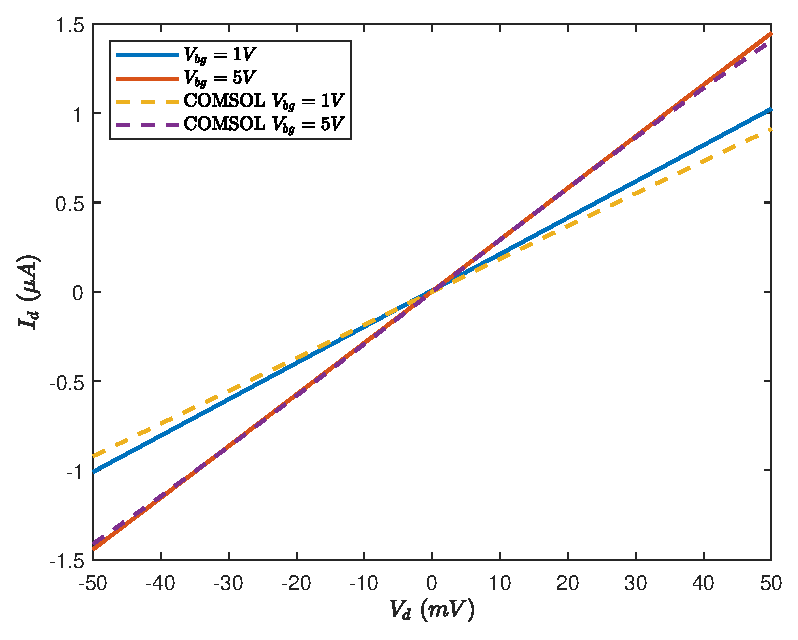
\includegraphics[width=.75\textwidth]{Grafici/Id(Vd)_HfO2_MoS2.eps} 
	\caption{$I_d(V_d)$ curve acquired for $V_{bg}$ values of 0, 1 and 5 V.}
	\label{fig:Id(Vd)_HfO2_MoS2}
\end{figure}

\begin{figure}[H]
	\centering
	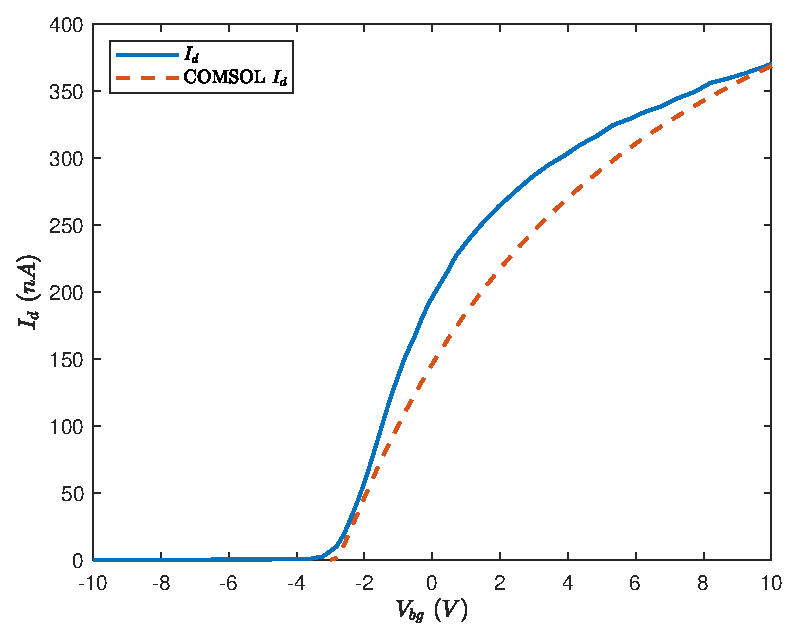
\includegraphics[width=.75\textwidth]{Grafici/Id(Vbg)_HfO2_MoS2.eps} 
	\caption{Transfer characteristic $I_d(V_{bg})$ for the FET with $10 mV$ applied bias voltage $V_{ds}$. Backgate voltage $V_{bg}$ is applied to the substrate and the top gate is disconnected.}
	\label{fig:Id(Vbg)_HfO2_MoS2}
\end{figure}

One of the crucial requirements for building integrated circuits based on single layers of MoS$_2$ is the ability to control charge density in a local manner, independently of a global back gate. We can do this by applying a voltage $V_{tg}$ to the top gate, separated from the monolayer MoS$_2$ by 30 nm of HfO$_2$ (Fig.~\ref{fig:HfO2_model}), while keeping the substrate grounded.

The corresponding transfer characteristic is shown in Fig.~\ref{fig:Id(Vtg)_HfO2_MoS2_varying_Vds}. For a bias of 10 mV we observe an on-current of 150 nA (37 $nA\mu m^{-1}$), current on/off ratio $I_{on}/I_{off} > 1 \cdot 10^6$ for the $\pm 4$ V range of $V_{tg}$ , an off-state current that is smaller than 100 fA (25 fA$\mu m^{-1}$) and gate leakage lower than 2 pA$\mu m^{-1}$. The observed current variation for different values of $V_{tg}$ indicates that the field-effect behaviour of our transistor is dominated by the MoS$_2$ channel and not the contacts.

At the bias voltage $V_{ds} = 500 mV$, the maximal measured on-current in~\cite{Radisavljevic:Si_MoS2} is 10 $\mu$A (2.5 mA $\mu m^{-1}$), with $I_{on}/I_{off} > 1 \cdot 10^8$ for the $\pm 4$ V range of $V_{tg}$. In our simulation for $V_{ds} = 500 mV$ the on-current is 3 $\mu$A but for  $V_{ds} = 100 mV$ and  $V_{ds} = 10 mV$ the on-current is the same as reported in the paper. 

\begin{figure}[H]
	\centering
	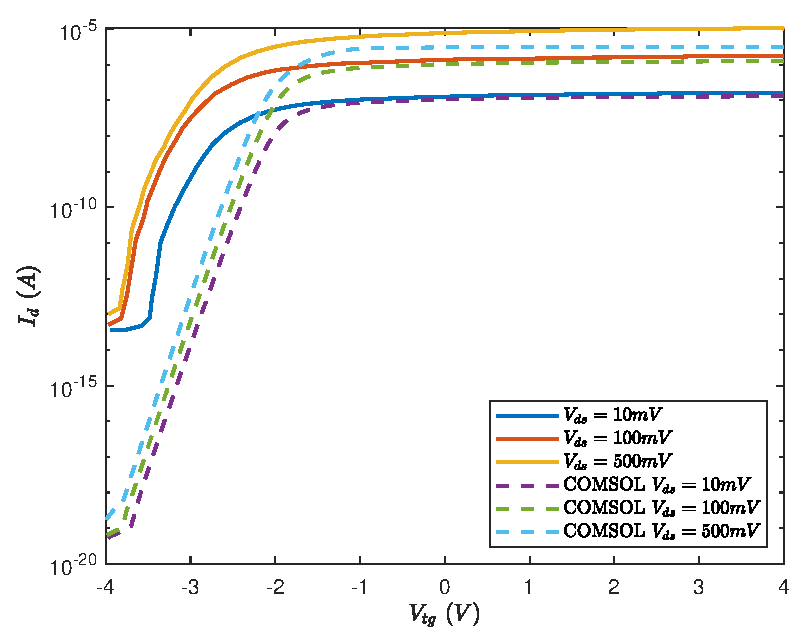
\includegraphics[width=1\textwidth]{Grafici/Id(Vtg)_HfO2_MoS2_varying_Vds.eps} 
	\caption{$I_{ds}$-$V_{tg}$ curve recorded for a bias voltage ranging from 10 mV to 500 mV. Measurements are performed with the back gate grounded. The device can be completely turned off by changing the top gate bias from –2 to –4 V. In~\cite{Radisavljevic:Si_MoS2} for $V_{ds} = 10 mV$ mV, the $I_{on}/I_{off}$ ratio is $10^6$. For $V_{ds} = 500 mV$, the $I_{on}/I_{off}$ ratio is $10^8$. We obtain a major value of $I_{on}/I_{off}$ ratio but we can still turn off the transistor with top gate bias from –2 to –4 V.}
	\label{fig:Id(Vtg)_HfO2_MoS2_varying_Vds}
\end{figure}

Fig.~\ref{fig:Id(Vtg)_HfO2_MoS2_varying_Vbg} shows the $I_{ds}$-$V_{tg}$ curve for $V_{bg}=0V$ and $V_{ds}=10mV$.

\begin{figure}[H]
	\centering
	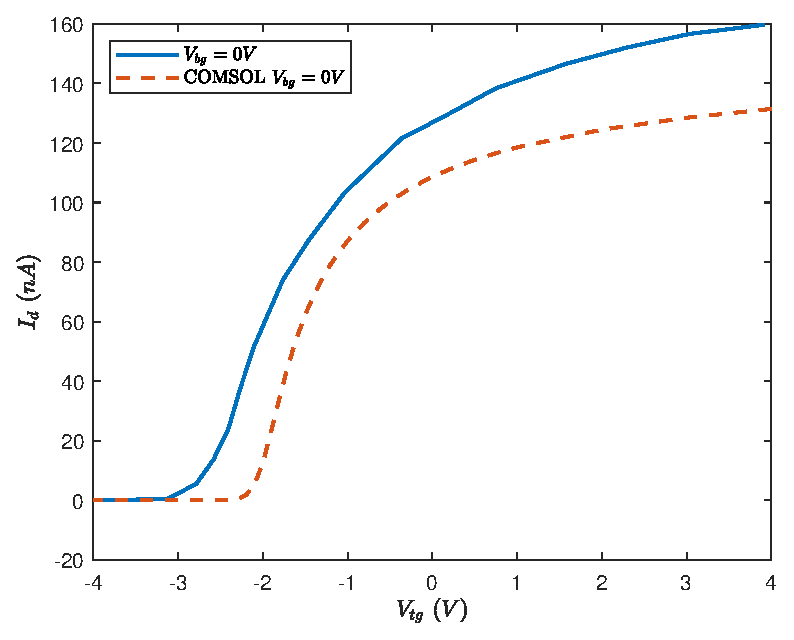
\includegraphics[width=1\textwidth]{Grafici/Id(Vtg)_HfO2_MoS2_varying_Vbg.eps} 
	\caption{$I_{ds}$-$V_{tg}$ for $V_{bg}=0V$.}
	\label{fig:Id(Vtg)_HfO2_MoS2_varying_Vbg}
\end{figure}

The large degree of current control in our device is also clearly illustrated in Fig.~\ref{fig:Id(Vds)_HfO2_MoS2_varying_Vtg}, where we plot the drain–source current versus drain–source bias for $V_{bg}=0V$.

\begin{figure}[H]
	\centering
	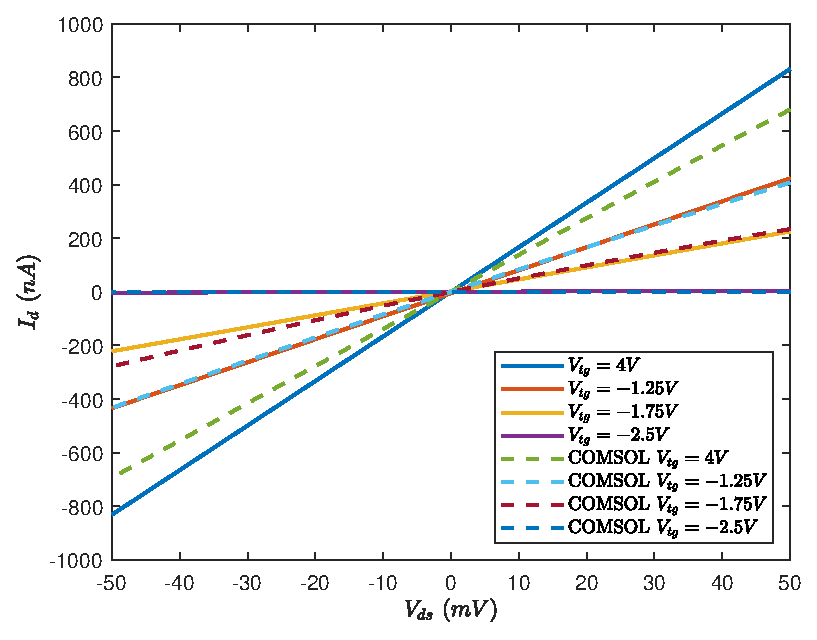
\includegraphics[width=1\textwidth]{Grafici/Id(Vds)_HfO2_MoS2_varying_Vtg.eps} 
	\caption{$I_d(V_{ds})$ curves recorded for different values of $V_{tg}$.}
	\label{fig:Id(Vds)_HfO2_MoS2_varying_Vtg}
\end{figure} 

\newpage
\section{MoS$_2$ transistor with Hf$_{0.3}$Zr$_{0.7}$O$_2$}
We tried to simulate a transitor with a thin layer of ferroelectric material. We used a layer of Hf$_{0.3}$Zr$_{0.7}$O$_2$ with 6 nm of thickness. We started from the previous COMSOL model, we changed the HfO$_2$ thickness from 30 nm to 20 nm.

\begin{figure}[H]
	\centering
	\includegraphics[width=.6\textwidth]{Immagini/HfZrO2_permittivity.png} 
	\caption{Hf$_{0.3}$Zr$_{0.7}$O$_2$ permittivity~\cite{Dragoman:ferroelectric}}
	\label{fig:HfZrO2_permittivity}
\end{figure}

We used the COMSOL interpolation model to implement the relation between the relative permittivity and the applied voltage described in~\cite{Dragoman:ferroelectric} and shown in~\ref{fig:HfZrO2_permittivity}. We used 10 points from the curve, a linear interpolation and a nearest function extrapolation. The result is shown in Fig.~\ref{fig:permittivity_HfZrO2}.

\begin{figure}[H]
	\centering
	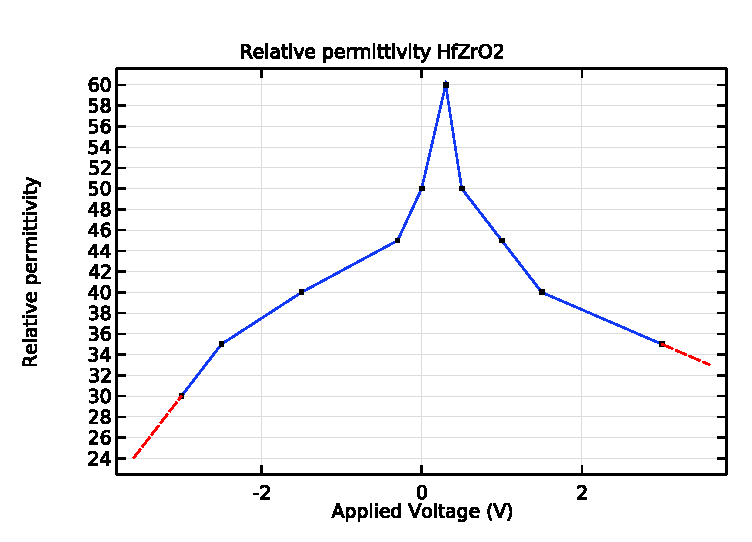
\includegraphics[width=.7\textwidth]{Grafici/permittivity_HfZrO2.eps} 
	\caption{COMSOL Hf$_{0.3}$Zr$_{0.7}$O$_2$ permittivity}
	\label{fig:permittivity_HfZrO2}
\end{figure}

We simulated the curves in COMSOL to see the FET behaviour. The Fig.~\ref{fig:HfZrO2_Id(Vd)_varying_Vbg} shows the $I_d$-$V_{ds}$ curve and is obtained with the top gate disconnected and for $V_{bg} = 0 V$ and $V_{bg} = 5 V$. We can see a resistive behaviour until $\sim1 $ V for $V_{bg} = 0 V$ and until $\sim3 $ V for $V_{bg} = 5 V$.
\begin{figure}[H]
	\centering
	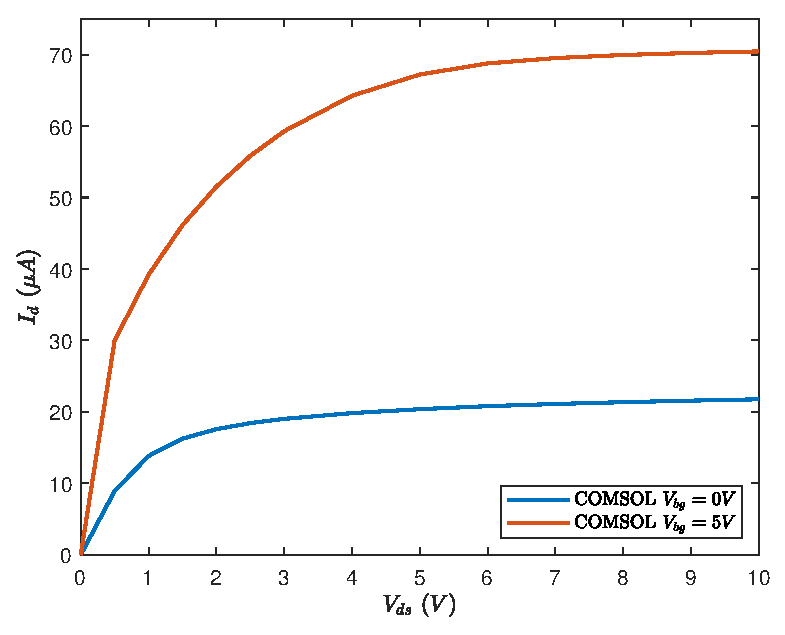
\includegraphics[width=.8\textwidth]{Grafici/HfZrO2_Id(Vd)_varying_Vbg.eps} 
	\caption{$I_d(V_{ds})$ varying $V_{bg}$}
	\label{fig:HfZrO2_Id(Vd)_varying_Vbg}
\end{figure} 

The Fig.~\ref{fig:HfZrO2_Id(Vd)_varying_Vtg} shows the $I_d$-$V_{ds}$ curve with $V_{bg} = 0$ for $V_{tg} = -2V$, $0V$ and $5V$. In this case the maximum drain current is about $25 \mu$A obtained for $V_{tg} = 5V$. In the resistive region the slope is greater that the previous study but the maximum current is lower.

\begin{figure}[H]
	\centering
	\includegraphics[width=.8\textwidth]{Grafici/HfZrO2_Id(Vd)_varying_Vtg.eps} 
	\caption{$I_d(V_{ds})$ varying $V_{tg}$}
	\label{fig:HfZrO2_Id(Vd)_varying_Vtg}
\end{figure} 

In Fig.~\ref{fig:HfZrO2_Id(Vtg)} is shown the $I_d$-$V_{tg}$ curve with $V_{bg}=0V$ and $V_{ds} = 10 mV$.

\begin{figure}[H]
	\centering
	\includegraphics[width=.8\textwidth]{Grafici/HfZrO2_Id(Vtg).eps} 
	\caption{$I_d(V_{tg})$}
	\label{fig:HfZrO2_Id(Vtg)}
\end{figure} 


\newpage

\nocite{*}
%Il comando \printbibliography produce la sezione bibliografica con relativi
%titolo e testatina. Per mandarne il relativo titolo nell’indice generale si
%usa l’istruzione:
\printbibliography

\end{document} 